\documentclass[]{article}
\usepackage[T1]{fontenc}
\usepackage[utf8]{inputenc}
\usepackage[french]{babel}
\usepackage{fullpage}
\usepackage{graphics}
\usepackage{graphicx}
\usepackage[center]{caption}
\usepackage{subcaption}
\usepackage{float}

\title{Simulation de particules sur architectures parallèles - version OpenCL}
\author{Alexis Couture, Marc Sarraute}

\begin{document}
\maketitle

\section{Bilan}

Pour ce second délivrable, nous avons implémenté une étape du tri par boite, la fonction scan, sous forme de noyau OpenCL (le reste du tri étant déjà implémenté). \\

On a réussi à implémenter un scan (ou prefix sum) qui s'exécute de manière parallèle. On a en entrée un tableau box\_buffer contenant le nombre d'atomes par boites et on écrit le résultat dans calc\_offset buffer. Notre fonction se déroule de la manière suivante :
\\

\begin{itemize}
\item On divise box\_buffer en le stockant par parties dans la mémoire locale de chaque workgroup, dans un tableau temp
\item Chaque workgroup réalise un prefix sum sur sa partie de box\_buffer, toujours sur temp
\item Chaque workgroup stocke la dernière valeur de son prefix sum dans box\_buffer (le workgroup i stocke son résultat dans la case i)
\item Chaque workgroup fait un prefix sum sur box\_buffer, et le stocke en mémoire locale dans le tableau local\_sumz
\item Chaque workgroup ajoute à son prefix sum, la somme des prefix sum obtenus par les workgroups précédents (traitant les parties antèrieures de box\_buffer)
\item On écrit les valeurs stockées dans temp dans calc\_offset\_buffer\\
\end{itemize}

Notre noyau utilise un thread par boite et partage le travail entre plusieurs workgroups. On utilise le tiling pour réduire, mais sans éliminer, le problème de dépendance inhérent à l'opération scan, où chaque thread a besoin du résultat du thread travaillant sur la case précédente. 
Au final, nous obtenons de moins bonnes performances qu'avec le tri par Z, signe que notre noyau est très perfectible.\\


\section{Limitations}

Tout d'abord, il n'existe pas en OpenCL de moyen propre pour synchroniser les workgroups entre eux car ceux-ci doivent travailler de manière indépendante. Pourtant, chaque workgroup a besoin des résultats des workgroups précédent pour "terminer" son calcul. Pour traiter ce problème, chaque workgroup stocke son résultat en mémoire globale dans box\_buffer, à la case d'indice de son group\_id, et récupère le résultat des autres workgroups sans vérifier si ceux-ci ont fini leur calcul. \\

Ensuite, notre implémentation a une complexité linéaire n + m (où n est le nombre de boites et m le nombre de workgroups) et utilise n threads (un thread par boite), ce qui n'est pas efficient. En conséquence, nous n'obtenons pas de performances supèrieures à celles du tri par Z version OpenCL, ce qui n'est pas satisfaisant étant donné que le tri par boite est théoriquement plus rapide. Une idée d'amélioration serait de suivre l'implémentation décrite par M. Harris\footnote{http://developer.download.nvidia.com/compute/cuda/1.1-Beta/x86\_website/projects/scan/doc/scan.pdf}, qui utilise moins de threads et possède une complexité logarithmique.\\

Enfin, notre kernel ne peut s'exécuter sur les plus grosses configurations (biochoc1 par exemple), en raison d'un grand nombre de boites. Là encore, on peut lier ce problème au grand nombre de threads utilisés mais aussi éventuellement à la quantité de mémoire locale utilisée, qui grandit avec le nombre de workgroups. 



\section{Tests}

Nous avons effectués des mesures de performances sur 2 machines différentes : 
\begin{itemize}
\item kira, doté d'un CPU de 12 coeurs hyperthreadés et d'un GPU NVIDIA Quadro K2000 (2 Go de RAM)
\item tesla, doté d'un CPU de 20 coeurs hyperthreadés et d'un GPU NVIDIA Tesla K20Xm (6 Go de RAM) \\
\end{itemize}
Pour résumer, la machine tesla dispose d'un bien meilleur GPU que kira, ce qui va permettre de déterminer si notre kernel tire parti du materiel ou non. 
On compare également 4 versions données ou implémentées :
\begin{itemize}
\item La version séquentielle, fournie au début du projet (uniquement sur kira)
\item La version OpenMP avec un tri par Z, implémentée lors de la première partie du projet, avec un nombre de threads dynamique (meilleurs résultats)
\item La version OpenCL avec un tri par Z, fournie pour la seconde partie du projet \\
... et la version OpenCL avec un tri par boite, dont on évalue les performances \\
\end{itemize}

En comparant les temps d'exécution sur différentes configurations, présentés sur les figures \ref{fig:histo-kira} et \ref{fig:histo-tesla}, on s'aperçoit que notre kernel gagne significativement en rapidité sur le meilleur support, tesla. Néanmoins, sur les 2 machines, la version OpenCL du tri par boites est toujours plus lente que la version OpenMP du tri par Z, signe que notre algorithme n'est vraiment pas optimal pour GPU.\\

En étudiant les résultats par configuration, on peut remarquer le résultat constant obtenu sur choc1, choc2, choc3 et choc4, qui s'explique par un nombre de boites identique entre ces 4 configurations. Comme nous l'avons dit précédemment, notre algorithme a une complexité linéaire liée au nombre de boites, ce qui explique ce résultat. Aussi, notre kernel ne peut pas s'exécuter sur la configuration biochoc1, qui contient bien plus de boites (et d'atomes), ce qui est assez regrettable.\\

\begin{figure}[H]
  \centering
  \includegraphics[scale=0.5]{Courbe/kira/histogram.png} 
  \caption{Comparaison entre les différentes versions sur plusieurs configurations - kira}
  \label{fig:histo-kira}
\end{figure}


\begin{figure}[H]
  \centering
  \includegraphics[scale=0.5]{Courbe/tesla/histo/histogram.png} 
  \caption{Comparaison entre les différentes versions sur plusieurs configurations - tesla}
  \label{fig:histo-tesla}
\end{figure}

Nous avons ensuite étudié les temps d'exécution de notre tri par boite et du tri par Z version OpenCL fourni, en fonction du nombre d'atomes strictement (résultats figure \ref{fig:atoms-tesla}). On y observe cette fois que notre tri par boite est bien plus rapide, avec une courbe qui augmente lentement par rapport au tri par Z. On peut expliquer ce changement de rapport de performances par le faible nombre de boites, qui induit une exécution plus rapide de notre kernel scan, et par le tri par Z, qui est théoriquement bien moins efficient que le tri par boites. \\

\begin{figure}[H]
  \centering
  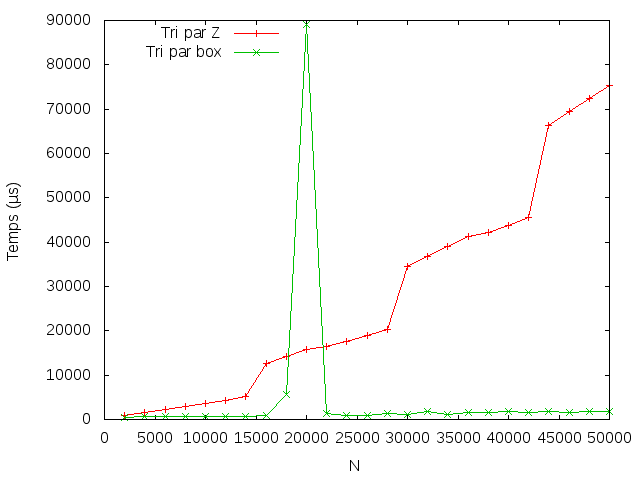
\includegraphics[scale=0.5]{Courbe/tesla/biochoc1/ocl_z-ocl_box.png} 
  \caption{Temps d'exécution du tri par boites et du tri par Z versions OpenCL, en fonction du nombre d'atomes, sur tesla}
  \label{fig:atoms-tesla}
\end{figure}

Au final, ces mesures montrent que notre kernel est très perfectible, au vue des performances obtenues par le tri par Z avec OpenCL.

\end{document}
